\documentclass[11pt,oneside]{book}
\usepackage{hyperref}
\usepackage{graphicx}
\usepackage{listings}
\usepackage{color}
\usepackage{tikz}
\usepackage[margin=1in]{geometry}
\usepackage{titlesec}
\usepackage{tcolorbox}
\usepackage{fancyhdr}
\usepackage{enumitem}

\titleformat{\chapter}{\normalfont\huge\bfseries}{\thechapter}{20pt}{\huge}
\titlespacing*{\chapter}{0pt}{-30pt}{20pt}

\pagestyle{fancy}
\fancyhf{}
\fancyhead[R]{\leftmark}
\fancyfoot[C]{\thepage}

\title{
    \Huge AP Computer Science Principles\\
    \Large Unofficial Summary\\[0.5em]
    \normalsize\textcolor{red}{Work in Progress - Under Development}
}
\author{\href{https://rowi.dev/}{Robin Wiethüchter}}
\date{\today}

\begin{document}
\maketitle

\begin{tcolorbox}[
    title=Disclaimer,
    colback=white,
    colframe=black,
    width=\textwidth-2cm,
    center
]
This is an \textit{unofficial} study resource not affiliated with College Board\textsuperscript{\textregistered} or Code.org\textsuperscript{\textregistered}. The content may:
\begin{itemize}[leftmargin=*,noitemsep]
    \item Contain errors or inaccuracies
    \item Deviate from official AP\textsuperscript{\textregistered} curriculum guidelines
    \item Not fully align with current exam requirements
    \item Be incomplete or outdated
\end{itemize}
Users should refer to official College Board\textsuperscript{\textregistered} materials for authoritative information.
\end{tcolorbox}

\tableofcontents

\chapter{Digital Information}

The foundation of computing lies in how computers represent and process information digitally. This unit explores how data is represented using binary and the implications of digital representation.

\section*{Learning Objectives}

\subsection*{Binary Numbers (2.1)}
\begin{itemize}[label=--]
    \item \textbf{DAT-1.A}: Explain how data can be represented using bits
    \item \textbf{DAT-1.B}: Explain the consequences of using bits to represent data
    \item \textbf{DAT-1.C}: Calculate and compare binary numbers
\end{itemize}

\subsection*{Data Compression (2.2)}
\begin{itemize}[label=--]
    \item \textbf{DAT-1.D}: Compare data compression algorithms in context
\end{itemize}

\subsection*{Legal and Ethical Concerns (5.5)}
\begin{itemize}[label=--]
    \item \textbf{IOC-1.F}: Explain how computing raises legal and ethical concerns
\end{itemize}

\section*{Essential Knowledge}

\subsection*{Binary and Data Representation}
\begin{itemize}
    \item \textbf{Basic Concepts}
        \begin{itemize}
            \item A bit (binary digit) is the smallest unit of data, representing either 0 or 1 % DAT-1.A.3
            \item A byte consists of 8 bits % DAT-1.A.4
            \item Computing devices represent all data digitally using bits at their lowest level % DAT-1.A.2
            \item Data values can be stored in variables, lists, or constants and can be used as input/output for procedures % DAT-1.A.1
        \end{itemize}
    
    \item \textbf{Data Abstraction}
        \begin{itemize}
            \item Abstraction reduces complexity by hiding irrelevant details while bringing together useful ones, allowing focus on the main idea % DAT-1.A.5
            \item Bits are grouped to represent higher-level abstractions like numbers, text, and colors % DAT-1.A.6
            \item The same bit sequence can mean different things in different contexts (e.g., the same bits might represent a number or a letter) % DAT-1.A.7
        \end{itemize}
        
    \item \textbf{Digital vs. Analog}
        \begin{itemize}
            \item Analog data has values that change smoothly over time (e.g., pitch and volume of music, colors in a painting, position of a runner) % DAT-1.A.8
            \item Digital data approximates analog data through sampling - measuring values at regular intervals to determine the bits needed for storage % DAT-1.A.9, DAT-1.A.10
        \end{itemize}
\end{itemize}

\begin{figure}[h]
    \centering
    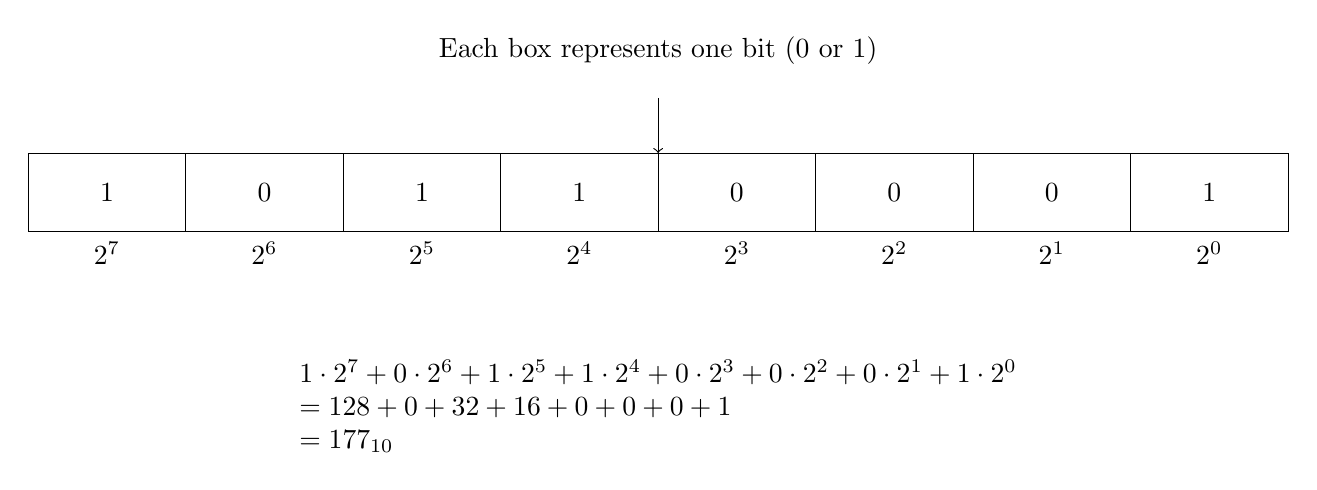
\begin{tikzpicture}[
        box/.style={
            draw,
            rectangle,
            minimum width=2cm,
            minimum height=1cm,
            align=center
        }
    ]
        % Binary representation boxes
        \foreach \x/\v in {0/1,1/0,2/1,3/1,4/0,5/0,6/0,7/1} {
            \node[box] at (\x*2,0) {\v};
        }
        
        % Labels
        \node[above] at (7,1.5) {Each box represents one bit (0 or 1)};
        \draw[->] (7,1.2) -- (7,0.5);
        
        % Power labels below
        \foreach \x/\p in {0/7,1/6,2/5,3/4,4/3,5/2,6/1,7/0} {
            \node[below] at (\x*2,-0.5) {$2^\p$};
        }
        
        % Add calculation below
        \node[below, align=left] at (7,-2) {
            $1 \cdot 2^7 + 0 \cdot 2^6 + 1 \cdot 2^5 + 1 \cdot 2^4 + 0 \cdot 2^3 + 0 \cdot 2^2 + 0 \cdot 2^1 + 1 \cdot 2^0$\\
            $= 128 + 0 + 32 + 16 + 0 + 0 + 0 + 1$\\
            $= 177_{10}$
        };
    \end{tikzpicture}
    \caption{Converting binary to decimal: Each bit's value is multiplied by its position value (powers of 2)}
    \label{fig:binary-byte}
\end{figure}

\begin{figure}[h]
    \centering
    \begin{tikzpicture}[
        box/.style={
            draw=none,
            minimum width=1cm,
            minimum height=0.8cm,
            align=center
        },
        carry/.style={
            font=\small,
            text=red
        }
    ]
        % Title
        \node[align=center] at (4,2) {Binary Addition Example};
        
        % First number
        \node[box] at (3,0) {1};
        \node[box] at (4,0) {0};
        \node[box] at (5,0) {1};
        \node[box] at (6,0) {1};
        
        % Plus sign and second number
        \node[box] at (1,-1) {+};
        \node[box] at (3,-1) {1};
        \node[box] at (4,-1) {0};
        \node[box] at (5,-1) {1};
        \node[box] at (6,-1) {1};
        
        % Carry numbers (just above the line)
        \node[carry] at (2,-1.3) {1};
        \node[carry] at (4,-1.3) {1};
        \node[carry] at (5,-1.3) {1};
        
        
        % Line
        \draw[thick] (1,-1.5) -- (6,-1.5);
        
        % Result
        % \node[box] at (2,-2) {1};
        \node[box] at (2,-2) {1};
        \node[box] at (3,-2) {0};
        \node[box] at (4,-2) {1};
        \node[box] at (5,-2) {1};
        \node[box] at (6,-2) {0};
        
        % Explanation
        \node[align=left] at (8,-3.5) {
            \hspace{1.0em}$11_{10} = \hspace{0.5em}1011_2$\\
            $+\: 11_{10} = \hspace{0.5em}1011_2$\\
            \hspace{1.0em}$22_{10} = 10110_2$
        };
        
    \end{tikzpicture}
    \caption{Binary addition example showing carry bits in red}
    \label{fig:binary-addition}
\end{figure}

\subsection*{Number Systems}
\begin{itemize}
    \item \textbf{Binary Numbers}
        \begin{itemize}
            \item Binary (base 2) uses only 0s and 1s % DAT-1.C.2
            \item Decimal (base 10) uses digits 0-9 % DAT-1.C.3
            \item A bit's position determines its value - multiply the bit (0 or 1) by the place value % DAT-1.C.4
            \item Place values are powers of 2, starting from right ($2^0$) and increasing leftward % DAT-1.C.5
        \end{itemize}
    
    \item \textbf{Limitations}
        \begin{itemize}
            \item Fixed-size integers in many programming languages have limited range, which can cause overflow errors % DAT-1.B.1
            \item Some languages allow unlimited integer size, limited only by computer memory % DAT-1.B.2
            \item Real numbers often have limited precision, leading to round-off errors when stored or calculated % DAT-1.B.3
        \end{itemize}
\end{itemize}

\subsection*{Data Compression}
\begin{itemize}
    \item \textbf{Basic Concepts}
        \begin{itemize}
            \item Data compression reduces the number of bits needed for data storage/transmission % DAT-1.D.1
            \item Fewer bits doesn't always mean less information % DAT-1.D.2
            \item Compression effectiveness depends on data redundancy and the algorithm used % DAT-1.D.3
        \end{itemize}

    \item \textbf{Types of Compression}
        \begin{itemize}
            \item Lossless: Guarantees exact reconstruction of original data % DAT-1.D.4
            \item Lossy: Creates approximation of original data, typically achieving better compression ratios % DAT-1.D.5, DAT-1.D.6
        \end{itemize}
    
    \item \textbf{Choosing Compression}
        \begin{itemize}
            \item Use lossless when exact reconstruction is crucial (e.g., text documents, program files) % DAT-1.D.7
            \item Use lossy when minimizing size/transmission time is priority (e.g., streaming video, music) % DAT-1.D.8
        \end{itemize}
\end{itemize}

\subsection*{Legal and Ethical Considerations}
\begin{itemize}
    \item \textbf{Intellectual Property}
        \begin{itemize}
            \item Digital content is the intellectual property of its creator or organization % IOC-1.F.1
            \item Digital distribution makes intellectual property concerns more complex % IOC-1.F.2
            \item Proper safeguards should protect intellectual property % IOC-1.F.3
            \item Using others' work without attribution is plagiarism with legal consequences % IOC-1.F.4
        \end{itemize}
    
    \item \textbf{Legal Usage}
        \begin{itemize}
            \item Creative Commons: Public license enabling free distribution of copyrighted work
            \item Open source: Programs freely available for redistribution and modification
            \item Open access: Research output free of access restrictions % IOC-1.F.5
            \item All borrowed material must be properly cited % IOC-1.F.6
        \end{itemize}

    \item \textbf{Broader Impact}
        \begin{itemize}
            \item Computing can affect social and political issues % IOC-1.F.9
            \item Digital divide raises ethical concerns about computing access % IOC-1.F.10
            \item Ethical concerns include biased algorithms, data collection privacy, and digital media access % IOC-1.F.11
        \end{itemize}
\end{itemize}
\chapter{The Internet}

\section*{Overview}
Exploration of Internet architecture, protocols, and its profound impact on modern society, including cultural, political, and economic implications.

% Key topics:
% - Network protocols
% - Internet architecture
% - Societal impacts 
% \chapter{Intro to App Design}

\section*{Overview}
Introduction to fundamental programming concepts through app development, emphasizing collaborative development practices and basic software design principles.

% Key topics:
% - Basic programming concepts
% - Software development lifecycle
% - Collaboration tools and practices 
% \chapter{Variables, Conditionals, and Functions}

\section*{Overview}
Core programming constructs that enable data storage, decision-making, and code organization, with emphasis on practical application in app development.

% Key topics:
% - Variable types and scope
% - Control structures
% - Function definition and usage 
% \chapter{Lists, Loops, and Traversals}

\section*{Overview}
Working with collections of data, implementing iteration, and processing data sequences to create more sophisticated applications.

% Key topics:
% - Data structures
% - Iteration methods
% - Data processing techniques 
% \chapter{Algorithms}

\section*{Overview}
Study of algorithm design, analysis, and evaluation, focusing on efficiency and problem-solving strategies.

% Key topics:
% - Algorithm analysis
% - Complexity considerations
% - Problem-solving approaches 
% \chapter{Parameters, Return, and Libraries}

\section*{Overview}
Advanced programming concepts focusing on code reusability, modularity, and the use of external libraries.

% Key topics:
% - Function parameters
% - Return values
% - Library integration 
% \chapter{Create PT Prep}

\section*{Overview}
Preparation and practice for the Create Performance Task, focusing on project development and documentation.

% Key topics:
% - Project planning
% - Implementation
% - Documentation requirements 
% \chapter{Data}

\section*{Overview}
Exploration of data analysis and visualization techniques, using real-world datasets to discover patterns and draw conclusions.

% Key topics:
% - Data analysis methods
% - Visualization techniques
% - Pattern recognition 
% \chapter{Cybersecurity and Global Impacts}

\section*{Overview}
Examination of cybersecurity principles and the broader implications of computing on society, including ethical considerations and policy impacts.

% Key topics:
% - Security principles
% - Ethics in computing
% - Social responsibility 

\bibliographystyle{plain}
\bibliography{references}

\end{document} 